% This file was created by tikzplotlib v0.9.7.
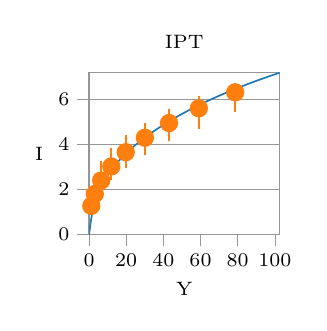
\begin{tikzpicture}
\scriptsize

\definecolor{color0}{rgb}{1,0.498039215686275,0.0549019607843137}
\definecolor{color1}{rgb}{0.12156862745098,0.466666666666667,0.705882352941177}

\begin{axis}[
axis line style={white!58.8235294117647!black},
height=0.3\textwidth,
tick align=outside,
tick pos=left,
title={IPT},
width=0.33\textwidth,
x grid style={white!58.8235294117647!black},
xlabel={Y},
xmin=0, xmax=102.56,
xtick style={color=white!58.8235294117647!black},
y grid style={white!58.8235294117647!black},
ylabel style={rotate=-90.0},
ylabel={I},
ymajorgrids,
ymin=0, ymax=7.18187462223965,
ytick style={color=white!58.8235294117647!black},
yticklabel style={anchor=east}
]
\path [draw=color0, semithick]
(axis cs:1.21,0.919189723601696)
--(axis cs:1.21,2.18028435365019);

\path [draw=color0, semithick]
(axis cs:3.126,1.35036487591379)
--(axis cs:3.126,2.69422770146139);

\path [draw=color0, semithick]
(axis cs:6.555,1.86440469480022)
--(axis cs:6.555,3.26591888412707);

\path [draw=color0, semithick]
(axis cs:12,2.40417588868152)
--(axis cs:12,3.86208817235529);

\path [draw=color0, semithick]
(axis cs:19.77,2.95098814706442)
--(axis cs:19.77,4.42054177606006);

\path [draw=color0, semithick]
(axis cs:30.05,3.52440771467503)
--(axis cs:30.05,4.96696794127002);

\path [draw=color0, semithick]
(axis cs:43.06,4.15853254448133)
--(axis cs:43.06,5.56389163621633);

\path [draw=color0, semithick]
(axis cs:59.1,4.69394682727128)
--(axis cs:59.1,6.1478586806875);

\path [draw=color0, semithick]
(axis cs:78.66,5.45545216758606)
--(axis cs:78.66,6.73670858328733);

\addplot [semithick, color1]
table {%
0 0
0.272000074386597 0.165183067321777
0.386000037193298 0.237001895904541
0.477999925613403 0.294456839561462
0.580999970436096 0.35909366607666
0.968999981880188 0.588913679122925
1.182000041008 0.703823685646057
1.38300001621246 0.804369926452637
1.55299997329712 0.883370637893677
1.73500001430511 0.962371110916138
1.9099999666214 1.0341899394989
2.2960000038147 1.17782747745514
2.57500004768372 1.27119183540344
2.95000004768372 1.38610184192657
3.28299999237061 1.47946619987488
3.64199995994568 1.57283055782318
4.02899980545044 1.66619491577148
4.38000011444092 1.74519550800323
4.78700017929077 1.83137798309326
5.18300008773804 1.9103786945343
5.60200023651123 1.98937928676605
6.00299978256226 2.06119799613953
6.73099994659424 2.18328976631165
7.375 2.28383612632751
8.11100006103516 2.39156413078308
8.84099960327148 2.49211049079895
9.61400032043457 2.59265685081482
10.4309997558594 2.69320297241211
11.2290000915527 2.7865674495697
12.1899995803833 2.89429545402527
12.8000001907349 2.95893239974976
13 2.98047804832458
14.2799997329712 3.10975170135498
14.6599998474121 3.14566111564636
15.0299997329712 3.18157052993774
17.9300003051758 3.44011783599854
18.6200008392334 3.49757289886475
18.8799991607666 3.51911854743958
21.5200004577637 3.72739291191101
22.2900009155273 3.78484797477722
22.6800003051758 3.81357550621033
25.4099998474121 4.00748586654663
26.4799995422363 4.07930469512939
26.9099998474121 4.1080322265625
29.3600006103516 4.26603364944458
30.6399993896484 4.34503412246704
31.1100006103516 4.37376165390015
34.0299987792969 4.54612684249878
39.4000015258789 4.84058332443237
43.6399993896484 5.05603981018066
49.0900001525879 5.31458711624146
53.939998626709 5.53004360198975
58.9199981689453 5.73831796646118
64.379997253418 5.95377397537231
69.379997253418 6.1405029296875
74.6399993896484 6.32723140716553
79.75 6.49959659576416
85.0999984741211 6.67196130752563
89.7699966430664 6.81559896469116
95.129997253418 6.97360038757324
100.209999084473 7.11723756790161
102.559997558594 7.18187475204468
};
\addplot [semithick, color0, mark=*, mark size=3, mark options={solid}, only marks]
table {%
1.21000003814697 1.27808225154877
3.12599992752075 1.80683207511902
6.55499982833862 2.40430331230164
12 3.02603125572205
19.7700004577637 3.65862703323364
30.0499992370605 4.30002593994141
43.060001373291 4.95149660110474
59.0999984741211 5.60632038116455
78.6600036621094 6.31477451324463
};
\end{axis}

\end{tikzpicture}
